\section{Domenemodell}

Beskrivelse av systemet med klassediagram, databasemodell og sekvensdiagram.

\subsection{Klassediagram}
For UML klasse diagram se vedlegg 1.
Diagrammet viser en grov skisse av hvordan klasser i applikasjonen skal defineres. Den beskriver også ulike interfaces som definerer funksjonalitet applikasjonen må ha for å kunne utføre oppgaver.

% ER - diagram
%\newpage
\subsection{ER-diagram}
\begin{figure}[ht]
    \centering
    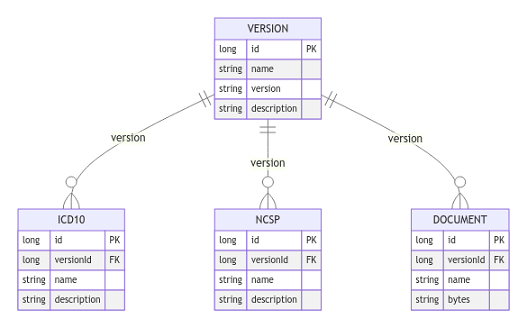
\includegraphics{images/ER2.png}
    \caption{ER - diagram. Generert med mermaid.}
    \label{fig:my_label}
\end{figure}

% Use Case diagram
%\subsection{Use Case diagram}

% Sequence diagram
\newpage
\subsection{Sekvensdiagram}
\begin{figure}[ht]
\centering
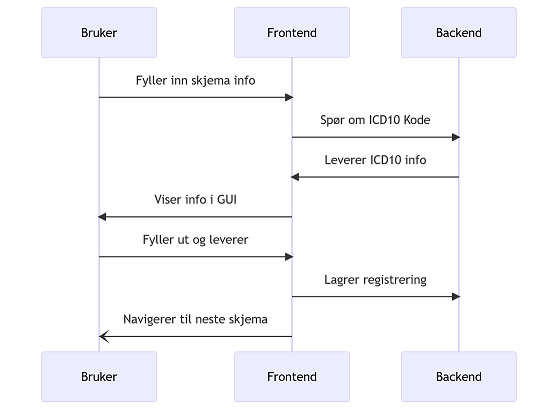
\includegraphics{images/sequence-diagram.png}
\caption{Sequence diagram. Generert med mermaid.}
\label{fig:sequence-diagram}
\end{figure}